\documentclass{beamer}
\usepackage{amsfonts,amsmath,amssymb,tikz}
\newcommand{\should}{\overset{\text{should}}{=}}
\newcommand{\fttheory}[1]{\fcolorbox{blue}{blue}{\color{white}\textbf{#1}\hspace{\textwidth}}}
\newcommand{\ftexampl}[1]{\fcolorbox{orange}{orange}{\color{black}\textbf{#1}\hspace{\textwidth}}}
\newcommand{\ftdata}[1]{\fcolorbox{violet}{violet}{\color{white}\textbf{#1}\hspace{\textwidth}}}
\newcommand{\ftheader}[1]{\fcolorbox{lightgray}{lightgray}{\color{black}\textbf{#1}\hspace{\textwidth}}}
\newcommand{\ftvocab}[1]{\fcolorbox{cyan}{cyan}{\color{black}\textbf{#1}\hspace{\textwidth}}}
\newcommand{\usd}{\text{ {\scriptsize USD}}}
\newcommand{\eur}{\text{ {\scriptsize EUR}}}
\newcommand{\aud}{\text{ {\scriptsize AUD}}}
\newcommand{\mxn}{\text{ {\scriptsize MXN}}}
\newcommand{\musd}{\text{ m {\scriptsize USD}}}
\newcommand{\meur}{\text{ m {\scriptsize EUR}}}
\newcommand{\maud}{\text{ m {\scriptsize AUD}}}

\begin{document}
%-----------------------------------------------------------------------------%
% STOCKS
%-----------------------------------------------------------------------------%

\begin{frame}{\ftheader{Stocks}}
	\begin{itemize}
		\item 
	\end{itemize}
\end{frame}

\begin{frame}
\begin{center}
	\Huge Observations 
\end{center}
\end{frame}

% dividend examples
\begin{frame}{\ftdata{Visa}}
	\begin{center}
		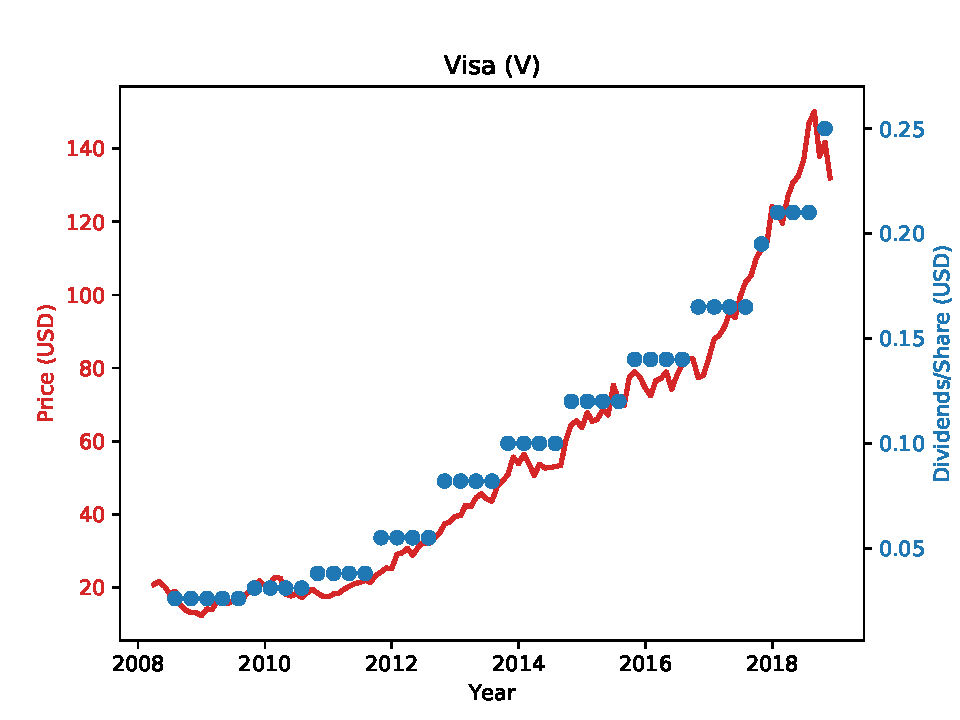
\includegraphics[scale=0.5]{V_col}
	\end{center}
\end{frame}

% dividend examples
\begin{frame}{\ftdata{Exxon}}
	\begin{center}
		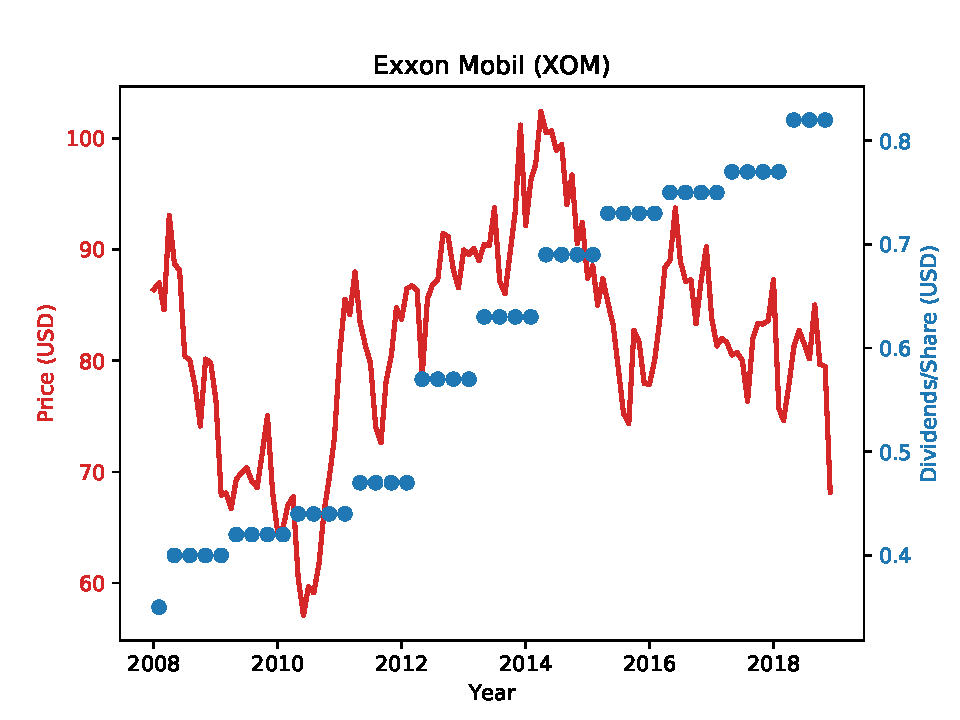
\includegraphics[scale=0.5]{XOM_col}
	\end{center}
\end{frame}

% dividend examples
\begin{frame}{\ftdata{Walmart}}
	\begin{center}
		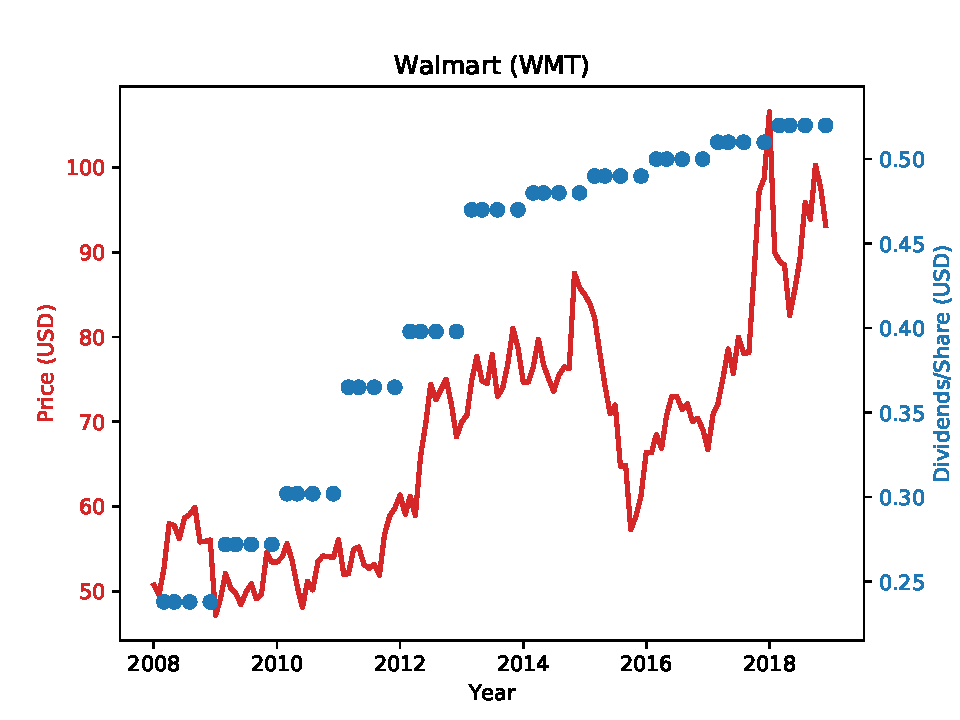
\includegraphics[scale=0.5]{WMT_col} 
	\end{center}
\end{frame}

% dividend examples
\begin{frame}{\ftdata{Observations}}
	\begin{itemize}
		\item Verizon's dividends are (generally) constant across the four quarters in each year, but increase from the fourth quarter of one year to the first quarter of the next
		\item Exxon's dividends follow a similar pattern to those of Verizon, despite the much greater volatility in its stock price
		\item Walmart's dividends follow a similar pattern to those of Verizon and Exxon, but the annual growth in the dividend rate seems to kink in 2013
	\end{itemize}
\end{frame}

\begin{frame}
	\begin{center}
		\Huge Stock Prices
	\end{center}
\end{frame}

% A One Year Investor
\begin{frame}{\fttheory{Stocks}}
	\begin{figure}[H]
		\begin{center}
			\begin{tikzpicture}
				\draw (0,0) -- (4,0);
				\foreach \x in {0,4}
					\draw(\x,-.1) -- (\x, .1);
				\draw (0,0) node[above=3pt] {0};
				\draw (4,0) node[above=3pt] {1};
				\draw (0,0) node[below=3pt] {$-P_{0}$};
				\draw (4,0) node[below=3pt] {$D_{1}+P_{1}$};
			\end{tikzpicture}
		\end{center}
	\end{figure}
	\begin{itemize}
		\item $P_{1}$ is the expected price in one period (usually one quarter)
		\item $r$ is the required total rate of return (usually quarterly)
		\item $D_{1}$ is the expected dividend 
		\item The price \underline{should} be
		\begin{equation*}
			P_{0}\should\frac{D_{1}+P_{1}}{1+r_{S}}.
		\end{equation*}
	\end{itemize}
\end{frame}

% Dividend Yields, Capital Gains, and Total Returns
\begin{frame}{\fttheory{Didend Yields, Capital Gains, and Total Returns}}
\begin{equation*}
r\should\frac{D_{1}+P_{1}}{P_{0}}-1=\underbrace{\frac{D_{1}}{P_{0}}}_{\text{Didend Yield}}+\underbrace{\frac{P_{1}-P_{0}}{P_{0}}}_{\text{Capital Gain Rate}}
\end{equation*}
\begin{itemize}
\item The \underline{dividend yield} is the expected annual dividend of the stock divided by its current price 
\item The \underline{capital gain rate} is the percent by which the stock price increases from the current period to the next
\item The \underline{total return} (or \underline{holding period return}) is the sum of the dividend yield and the capital gain rate  
\end{itemize}
\end{frame}

% A Multiyear Investor
\begin{frame}{\fttheory{Stocks}}
	\begin{figure}[H]
		\begin{center}
			\begin{tikzpicture}
				\draw (0,0) -- (8,0);
				\foreach \x in {0,4,8}
				\draw(\x cm,3pt) -- (\x cm, -3pt);
				\draw (0,0) node[above=3pt] {0};
				\draw (4,0) node[above=3pt] {1};
				\draw (8,0) node[above=3pt] {2};
				\draw (0,0) node[below=3pt] {$-P_{0}$};
				\draw (4,0) node[below=3pt] {$D_{1}$};
				\draw (8,0) node[below=3pt] {$D_{2}+P_{2}$};
			\end{tikzpicture}
		\end{center}
	\end{figure}
\begin{itemize}
\item The prices should be
\begin{equation*}
	P_{0}\should\frac{D_{1}}{1+r_{S}}+\frac{D_{2}+P_{2}}{(1+r_{S})^2}\text{ and } P_{1}\should\frac{D_{2}+P_{2}}{1+r_{S}}.
\end{equation*}
\item Does the two-year investor value the stock differently than the one-ear investor? \textbf{No!}
\begin{equation*}
	P_{0}=\frac{D_{1}}{1+r_{S}}+\frac{D_{2}+P_{2}}{(1+r_{S})^2}=\frac{D_{1}}{1+r_{S}}+\frac{P_{1}}{1+r_{S}}=\frac{D_{1}+P_{1}}{1+r_{S}}
\end{equation*}
\end{itemize}
\end{frame}

% Dividend Discount Model Equation
\begin{frame}{\fttheory{The Dividend Discount Model}}
	\begin{itemize}
		\item It doesn't matter whether the investor wants to hold the stock for one quarter, two quarters, or infinitely many quarters: she is always willing to pay the same price $P_{0}$
		\item In particular, the investor who holds the stock for infinitely many periods is willing to pay 
		\begin{equation*}
			P_{0}\should\frac{D_{1}}{1+r_{S}}+\frac{D_{2}}{(1+r_{S})^2}+\frac{D_{3}}{(1+r_{S})^3}+\cdots 
		\end{equation*}
		for the stock
		\item Implication: we don't need to know the prices $P_{1}$, $P_{2}$, $\ldots$, just the dividends $D_{1}$, $D_{2}$, $D_{3}$, $\ldots$
	\end{itemize}
\end{frame}

% Growing Perpetuities
\begin{frame}{\fttheory{Constant Dividend Growth}}
Simple model: dividends grow at a constant rate $g$ 
\begin{figure}[H]
	\begin{center}
		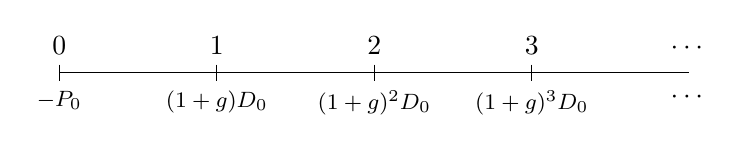
\begin{tikzpicture}
		\draw (0,0) -- (8,0);
		\foreach \x in {0,2,4,6}
		\draw(\x cm,3pt) -- (\x cm, -3pt);
		\draw (0,0) node[above=3pt] {0};
		\draw (2,0) node[above=3pt] {1};
		\draw (4,0) node[above=3pt] {2};
		\draw (6,0) node[above=3pt] {3};
		\draw (0,0) node[below=3pt] {};
		\draw (0,0) node[below=3pt] {\footnotesize$-P_{0}$};
		\draw (2,0) node[below=3pt] {\footnotesize$(1+g)D_{0}$};
		\draw (4,0) node[below=3pt] {\footnotesize$(1+g)^{2}D_{0}$};
		\draw (6,0) node[below=3pt] {\footnotesize$(1+g)^{3}D_{0}$};
		\draw (8,0) node[above=3pt, align=center] {$\cdots$};
		\draw (8,0) node[below=3pt, align=center] {$\cdots$};
		\end{tikzpicture}
	\end{center}
\end{figure}
where $D_{0}$ is the dividend that was \underline{just} paid
\begin{equation*}
	P_{0}\should\frac{(1+g)D_{0}}{(1+r_{S})}+\frac{(1+g)^{2}D_{0}}{(1+r_{S})^2}+\frac{(1+g)^{3}D_{0}}{(1+r_{S})^3}+\cdots=\frac{(1+g)D_{0}}{r_{S}-g}
\end{equation*}
\end{frame}

% Constant Dividend Growth
\begin{frame}{\fttheory{Constant Dividend Growth}}
\begin{itemize}
	\item The Dividend Discount Model says that
	\begin{equation*}
		P_{0}\should\frac{(1+g)D_{0}}{r_{S}-g}=\frac{D_{1}}{r_{S}-g}
	\end{equation*}
	\item Awesome interpretation!
	\begin{equation*}
		\overbrace{\frac{D_{1}}{P_{0}}+g}^{\text{Specific Formula}}\should r\should\overbrace{\underbrace{\frac{D_{1}}{P_{0}}}_{\text{Didend Yield}}+\underbrace{\frac{P_{1}-P_{0}}{P_{0}}}_{\text{Capital Gain Rate}}}^{\text{General Formula}}
	\end{equation*}
	\item In this case, the \underline{growth rate} $g$ is the \underline{capital gain rate}
\end{itemize}
\end{frame}

\begin{frame}
\begin{center}
\Huge Price-to-Earnings Ratios
\end{center}
\end{frame}

\begin{frame}{\fttheory{Price-to-Earnings (P/E) Ratios}}
\begin{itemize}
	\item Unfortunately, computing prices via DCF can be extremely complicated and prone to error as one must be able to forecast the firm's payout policies, how those payouts correlate with the performance of the market, and so on
	\item In practice, finance professionals often use \underline{multiples} to price stocks (or entire companies)
\end{itemize}
\end{frame}

\begin{frame}{\fttheory{Price-to-Earnings (P/E) Ratios}}
\begin{itemize}
	\item Suppose that companies $A$ and $B$ have similar risk ($\beta_{A}\approx\beta_{B}$) and hence similar expected returns ($\text{E}[r_{A}]\approx\text{E}[r_{B}]$)
	\item P/E valuation assumes that earnings equal dividends: $E_{A}=D_{A}$ and $E_{B}=D_{B}$. 
	\item Then $A$ and $B$ should have the same P/E ratio:
	\begin{equation}
		\frac{P_{A}}{E_{A}}\approx\frac{P_{B}}{E_{B}}
	\end{equation}
	\item If we know $B$'s P/E ratio and $A$'s earnings-per-share, we can approximate $A$'s price:
	\begin{equation}
		P_{A}\approx E_{A}\times\frac{P_{B}}{E_{B}}
	\end{equation}
	\item In this case, $P_{B}/E_{B}$ is the \textit{multiple}
\end{itemize}
\end{frame}

\begin{frame}{\ftexampl{Price-to-Earnings (P/E) Ratios}}
\begin{itemize}
	\item Suppose that we want to price Honeywell (HON), which has a beta of 1.08. Lockheed Martin (LMT) has a beta of 0.93, while Walmart has a beta of 0.29. We should use the multiple of which company?
	\pause
	\item {\color{blue} Lockheed Martin. It's beta (and hence expected return) is much closer to that of Honeywell than that of Walmart.}
\end{itemize}
\end{frame}

\begin{frame}{\ftexampl{Price-to-Earnings (P/E) Ratios}}
\begin{center}
	\begin{tabular}{lllll}
		\textbf{Stock} & \textbf{Beta} & \textbf{P} & \textbf{E}(PS) & \textbf{P/E} \\ 
		Honeywell & & & & 8.14 \\
		Lockheed & & 386.70 & 22.82 & 16.95 \\
	\end{tabular}
\end{center}
\begin{itemize}
	\item What should Honeywell trade for?
	\pause
	\item {\color{blue}
		\begin{equation}
			P_{\text{HON}}\approx E_{\text{HON}}\times\frac{P_{\text{LMT}}}{E_{\text{LMT}}}=8.14\text{ USD}\times\frac{386.70\text{ USD}}{22.82\text{ USD}}=
		\end{equation}
	}
	\item {\color{blue} Honeywell was \textit{actually} trading for 161.49}
\end{itemize}
\end{frame}

\begin{frame}{Notes for Jordan (and the curious student)}
The SDF
\begin{equation}
	m(1+r_{f})=1-\text{SR}[r_{m}]z_{m}
\end{equation}
prices the return of the total endowment, $r_{m}$, and the risk-free rate, $r_{f}$, where $z_{m}=(r_{m}-\text{E}[r_{m}])/\text{SD}[r_{m}]$. So if the stock's dividends grow at a random rate of $g$, then
\begin{align}
	P_{0}&=\sum_{k=1}^{\infty}{\text{E}\left[(m(1+g))^{k}\right]D_{0}}\\
	&=\sum_{k=1}^{\infty}{\frac{\text{E}\left[((1-\text{SR}[r_{m}]z_{m})(1+g))^{k}\right]D_{0}}{(1+r_{f})^k}}
\end{align}
\end{frame}
\end{document}
